\documentclass[11pt,a4paper]{article}
\usepackage{vntex}
%\usepackage[english,vietnam]{babel}
%\usepackage[utf8]{inputenc}

%\usepackage[utf8]{inputenc}
%\usepackage[francais]{babel}
\usepackage{a4wide,amssymb,epsfig,latexsym,array,hhline,fancyhdr}

\usepackage{amsmath}
\usepackage{amsthm}
\usepackage{multicol,longtable,amscd}
\usepackage{diagbox}%Make diagonal lines in tables
\usepackage{booktabs}
\usepackage{alltt}
\usepackage[framemethod=tikz]{mdframed}% For highlighting paragraph backgrounds
\usepackage{caption,subcaption}

\usepackage{lastpage}
\usepackage[lined,boxed,commentsnumbered]{algorithm2e}
\usepackage{enumerate}
\usepackage{color}
\usepackage{graphicx}							% Standard graphics package
\usepackage{array}
\usepackage{tabularx, caption}
\usepackage{multirow}
\usepackage{multicol}
\usepackage{rotating}
\usepackage{graphics}
\usepackage{geometry}
\usepackage{setspace}
\usepackage{epsfig}
\usepackage{tikz}
\usetikzlibrary{arrows,snakes,backgrounds}
\usepackage[unicode]{hyperref}
\hypersetup{urlcolor=blue,linkcolor=black,citecolor=black,colorlinks=true} 
%\usepackage{pstcol} 								% PSTricks with the standard color package

\newtheorem{theorem}{{\bf Định lý}}
\newtheorem{property}{{\bf Tính chất}}
\newtheorem{proposition}{{\bf Mệnh đề}}
\newtheorem{corollary}[proposition]{{\bf Hệ quả}}
\newtheorem{lemma}[proposition]{{\bf Bổ đề}}


%\usepackage{fancyhdr}
\setlength{\headheight}{40pt}
\pagestyle{fancy}
\fancyhead{} % clear all header fields
\fancyhead[L]{
 \begin{tabular}{rl}
    \begin{picture}(25,15)(0,0)
    \put(0,-8){
\includegraphics[width=8mm, height=8mm]{Images/hcm.png}}
    %\put(0,-8){\epsfig{width=10mm,figure=hcmut.eps}}
   \end{picture}&
	%
\includegraphics[width=8mm, height=8mm]{hcm.png} & %
	\begin{tabular}{l}
		\textbf{\bf \ttfamily Trường Đại Học Bách Khoa Tp.Hồ Chí Minh}\\
		\textbf{\bf \ttfamily Khoa Khoa Học và Kỹ Thuật Máy Tính}
	\end{tabular} 	
 \end{tabular}
}
\fancyhead[R]{
	\begin{tabular}{l}
		\tiny \bf \\
		\tiny \bf 
	\end{tabular}  }
\fancyfoot{} % clear all footer fields
\fancyfoot[L]{\scriptsize \ttfamily Bài tập lớn môn Trí tuệ nhân tạo - Niên khóa 2017-2018}
\fancyfoot[R]{\scriptsize \ttfamily Trang {\thepage}/\pageref{LastPage}}
\renewcommand{\headrulewidth}{0.3pt}
\renewcommand{\footrulewidth}{0.3pt}


%%%
\setcounter{secnumdepth}{4}
\setcounter{tocdepth}{3}
\makeatletter
\newcounter {subsubsubsection}[subsubsection]
\renewcommand\thesubsubsubsection{\thesubsubsection .\@alph\c@subsubsubsection}
\newcommand\subsubsubsection{\@startsection{subsubsubsection}{4}{\z@}%
                                     {-3.25ex\@plus -1ex \@minus -.2ex}%
                                     {1.5ex \@plus .2ex}%
                                     {\normalfont\normalsize\bfseries}}
\newcommand*\l@subsubsubsection{\@dottedtocline{3}{10.0em}{4.1em}}
\newcommand*{\subsubsubsectionmark}[1]{}
\makeatother

\everymath{\color{blue}}%make in-line maths symbols blue to read/check easily

\sloppy
\captionsetup[figure]{labelfont={small,bf},textfont={small,it},belowskip=-1pt,aboveskip=-9pt}
%space remove between caption, figure, and text
\captionsetup[table]{labelfont={small,bf},textfont={small,it},belowskip=-1pt,aboveskip=7pt}
%space remove between caption, table, and text

%\floatplacement{figure}{H}%forced here float placement automatically for figures
%\floatplacement{table}{H}%forced here float placement automatically for table
%the following settings (11 lines) are to remove white space before or after the figures and tables
%\setcounter{topnumber}{2}
%\setcounter{bottomnumber}{2}
%\setcounter{totalnumber}{4}
%\renewcommand{\topfraction}{0.85}
%\renewcommand{\bottomfraction}{0.85}
%\renewcommand{\textfraction}{0.15}
%\renewcommand{\floatpagefraction}{0.8}
%\renewcommand{\textfraction}{0.1}
\setlength{\floatsep}{5pt plus 2pt minus 2pt}
\setlength{\textfloatsep}{5pt plus 2pt minus 2pt}
\setlength{\intextsep}{10pt plus 2pt minus 2pt}

\begin{document}

\begin{titlepage}
\begin{center}
ĐẠI HỌC QUỐC GIA THÀNH PHỐ HỒ CHÍ MINH \\
TRƯỜNG ĐẠI HỌC BÁCH KHOA \\
KHOA KHOA HỌC - KỸ THUẬT MÁY TÍNH 
\end{center}

\vspace{1cm}

\begin{figure}[h!]
\begin{center}

\includegraphics[width=5cm]{Images/hcm.png}
\end{center}
\end{figure}

\vspace{1cm}


\begin{center}
\begin{tabular}{c}
\multicolumn{1}{l}{\centerline{\textbf{{\Large BÀI TẬP LỚN 1 }}}}\\
\textbf{{\Huge TÌM KIẾM (SEARCHING)}}\\
~~\\
\hline
\\
%\multicolumn{1}{l}{\textbf{{\Large Nhóm: ... ---- Bài tập lớn}}}\\
\\
%\textbf{\huge Phân tích yêu cầu và thiết kế kiến trúc: AgriExtension}\\
\textbf{{\Huge Môn Nhập môn trí tuệ nhân tạo}} \\
\\
\hline
\\
\end{tabular}
\end{center}

\vspace{1cm}

\begin{table}[h]
\begin{tabular}{rrl}
\hspace{5 cm} & GVHD: & Vương Bá Thịnh\\

& SV thực hiện: & Nguyễn Văn Thi -- 1513164 \\
& & Nguyễn Tuyết Nga -- 1512111 \\
\end{tabular}
\end{table}

\vspace{0.75cm}
\begin{center}
{\footnotesize Tp. Hồ Chí Minh, Tháng 5/2018}
\end{center}
\end{titlepage} 

\tableofcontents
\newpage
\section {Depth First Search}
\subsection{Giải thuật}
\begin{flushleft}
\hspace{2 cm}	def depth\_first\_search(initState, maxdepth = 50):\\
\hspace{3 cm}	initState.getMap().name +="(depth first search)"\\
\hspace{3 cm}	counter = 0\\
\hspace{3 cm}	stack = list()\\
\hspace{3 cm}	explored = list()\\
\hspace{3 cm}	stack.append(initState)\\
\hspace{3 cm}	while stack:\\
\hspace{4 cm}	state = stack.pop()\\
\hspace{4 cm}	check, value = state.isGoal()\\
\hspace{4 cm}	counter += 1\\
\hspace{4 cm}	if check == True:\\
\hspace{5 cm}	if value == None:\\
\hspace{6 cm}	return [state, counter]\\
\hspace{4 cm}	explored.append(state)\\
\hspace{4 cm}	if state.value > maxdepth:\\
\hspace{5 cm}	continue\\
\hspace{4 cm}	children = nextState(state)\\
\hspace{4 cm}	for i in children:\\
\hspace{5 cm}	if i not in explored:\\
\hspace{6 cm}	stack.append(i)\\
\hspace{3 cm}	return [initState, -1]\\
\end{flushleft}
\newpage
\subsection{Kết quả chi tiết từng bài}
\begin{center}
	\begin{tabular}{|c|r|c|c|c|}
		\hline
		Bài & Thời gian tìm kiếm kết quả & Chiều cao & Bước chuyển & Trạng thái \\ \hline
		1   & 0.250633 s	& 50	& 50	& 73 \\ \hline
		2   & 1.285382 s	& 100	& 101	& 230 \\ \hline
		3	& 0.406117 s	& 50 	& 47	& 66 \\ \hline
		4 	& 0.576354 s	& 50	& 40	& 76 \\ \hline
		5	& 1.385429 s	& 100	& 91	& 143\\ \hline
		6	& 0.762524 s	& 100	& 58	& 81 \\ \hline
		7	& 1.087740 s	& 100	& 66	& 144 \\ \hline
		8	& 0.577750 s	& 50	& 48	& 88 \\ \hline
		9	& 0.505913 s	& 100	& 65	& 96 \\ \hline
		10	& 1.652326 s	& 100	& 93	& 169 \\ \hline
		11	& 0.481144 s	& 50	& 49	& 65 \\ \hline
		12	& 3.030183 s	& 100	& 91	& 372 \\ \hline
		13	& 1.237571 s	& 100	& 65	& 134 \\ \hline
		14	& 3.403988 s	& 200	& 125	& 372 \\ \hline
		15	& 3.878507 s	& 100	& 82	& 370 \\ \hline
		16	& 0.636102 s	& 50	& 50	& 96 \\ \hline
		17	& 7.143340 s	& 300	& 295	& 698 \\ \hline
		18	& 1.643250 s	& 100	& 98	& 176 \\ \hline
		19	& 1.559267 s	& 100	& 87	& 154 \\ \hline
		20	& Not found		& 0		& 0		& -1 \\ \hline
		21	& 1.421129 s	& 100	& 72	& 179 \\ \hline
		22	& 2.075379 s	& 200	& 124	& 223 \\ \hline
		23	& 57.001248 s	& 300	& 301	& 4060 \\ \hline
		24	& 0.941831 s	& 100	& 82	& 123 \\ \hline
		25	& 2.173283 s	& 100	& 97	& 209 \\ \hline
		26	& 3.384305 s	& 200	& 150	& 310 \\ \hline
		27	& 2.548648 s	& 100	& 93	& 255 \\ \hline
		28	& 2.133764 s	& 200	& 120	& 214 \\ \hline
		29	& 21.487838 s	& 200	& 168	& 1609 \\ \hline
		30	& 3.033576 s	& 200	& 130	& 278 \\ \hline
		31	& 4.277469 s	& 200	& 195	& 423 \\ \hline
		32	& 2.301186 s	& 200	& 144	& 224 \\ \hline
		33	& 3.359139 s	& 200	& 96	& 284 \\ \hline	
	\end{tabular}	
\end{center}
\newpage
\subsection{Cách chạy} 
\begin{flushleft}
	\hspace{2 cm}	Bước 1: Chạy lệnh python3 src/Bloxor.py để vào chương trình
\end{flushleft}
\begin{center}
	\begin{figure}[htp]
		\begin{center}
			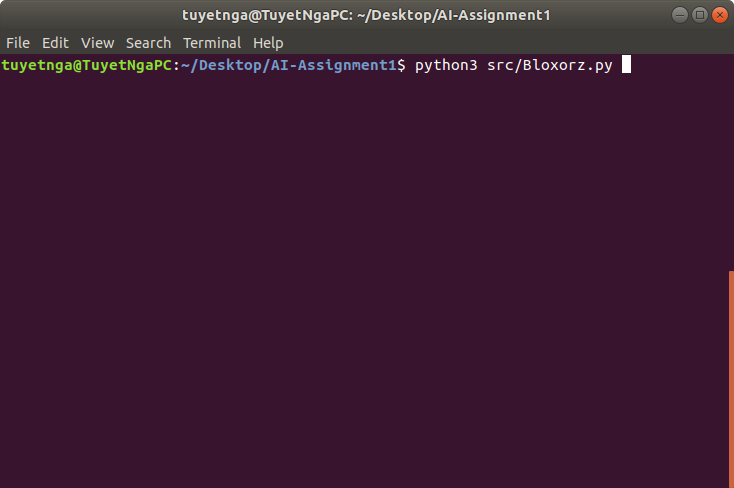
\includegraphics[width=10cm]{Images/depth1.png}
		\end{center}
		\caption{\label{fig:depth1}}
	\end{figure}
\end{center}
\begin{flushleft}
	\hspace{2 cm} Bước 2: Nhập bàn muốn chơi
\end{flushleft}
\begin{center}
	\begin{figure}[htp]
		\begin{center}
			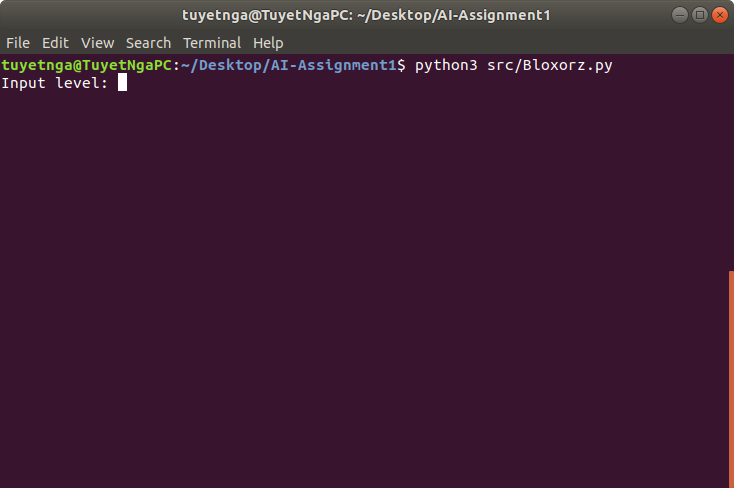
\includegraphics[width=10cm]{Images/depth2.png}
		\end{center}
		\caption{\label{fig:depth2}}
	\end{figure}
\end{center}
\newpage
\begin{flushleft}
	\hspace{3 cm} Bước 3: Nhập 2 để chọn giải thuật Depth First Search
\end{flushleft}
\begin{center}
	\begin{figure}[htp]
		\begin{center}
			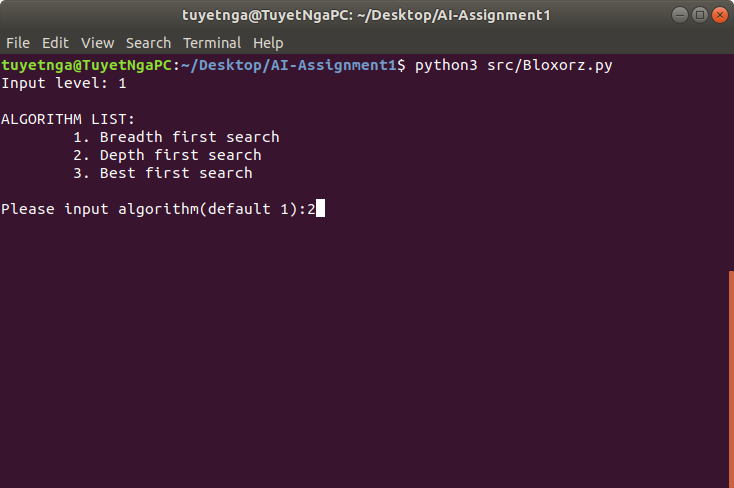
\includegraphics[width=10cm]{Images/depth3.png}
		\end{center}
		\caption{\label{fig:depth3}}
	\end{figure}
\end{center}
\begin{flushleft}
	\hspace{2 cm}	Bước 4: Nhập chiều dài của cây để giới hạn thời gian chạy
\end{flushleft}
\begin{center}
	\begin{figure}[htp]
		\begin{center}
			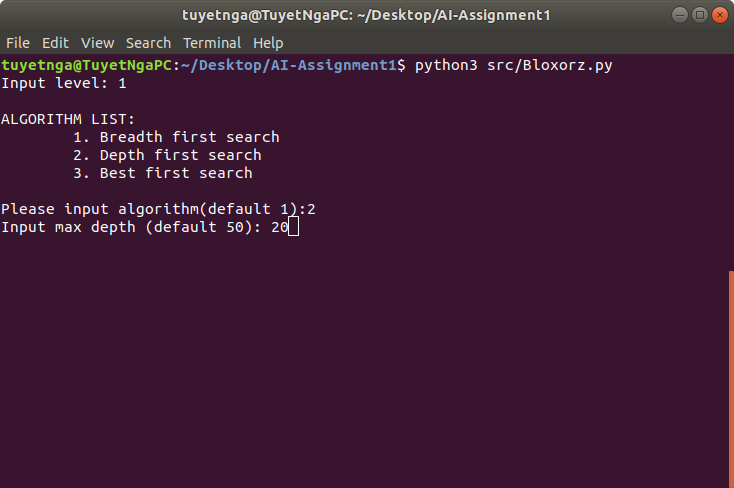
\includegraphics[width=10cm]{Images/depth4.png}
		\end{center}
		\caption{\label{fig:depth4}}
	\end{figure}
\end{center}
\newpage
\begin{flushleft}
	\hspace{2 cm}	Bước 5: Demo step-by-step, trong đó có tổng các trạng thái tìm được, lời giải tốt nhất và thời gian chạy
\end{flushleft}
\begin{center}
	\begin{figure}[htp]
		\begin{center}
			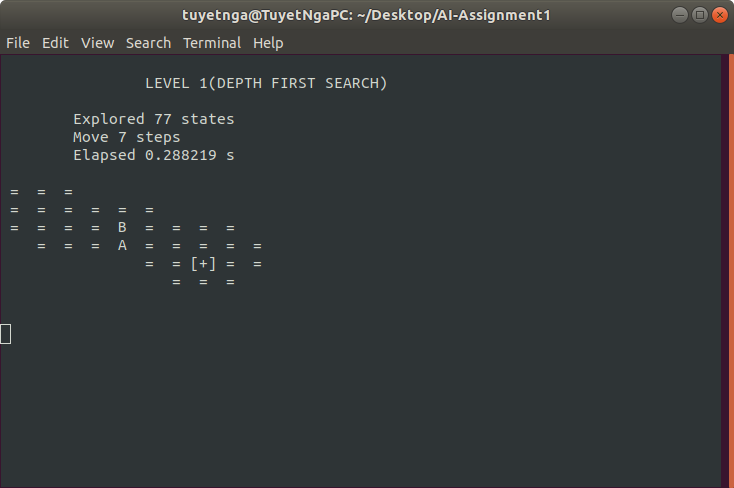
\includegraphics[width=10cm]{Images/depth5.png}
		\end{center}
		\caption{\label{fig:depth5}}
	\end{figure}
\end{center}
\begin{flushleft}
	\hspace{2 cm}	Bước 6: Xuất bước chạy rõ hơn sau khi đã có kết quả
\end{flushleft}
\begin{center}
	\begin{figure}[htp]
		\begin{center}
			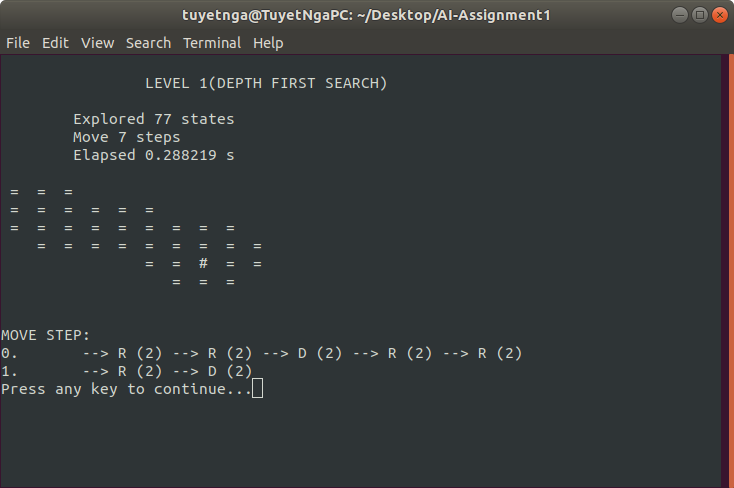
\includegraphics[width=10cm]{Images/depth6.png}
		\end{center}
		\caption{\label{fig:depth6}}
	\end{figure}
\end{center}
\newpage

\section{Breadth First Search}
\subsection{Giải thuật}
\begin{flushleft}
	\hspace{2 cm}	def breadth\_first\_search(initState):\\
	\hspace{3 cm}	initState.getMap().name +="(breadth first search)"\\
	\hspace{3 cm}	counter = 0\\
	\hspace{3 cm}	queue = list()\\
	\hspace{3 cm}	explored = list()\\
	\hspace{3 cm}	queue.append(initState)\\
	\hspace{3 cm}	while queue:\\
	\hspace{4 cm}	state = queue.pop(0)\\
	\hspace{4 cm}	check, value = state.isGoal()\\
	\hspace{4 cm}	counter += 1\\
	\hspace{4 cm}	explored.append(state)\\
	\hspace{4 cm}	if check == True:\\
	\hspace{5 cm}	queue.clear()\\
	\hspace{5 cm}	explored.clear()\\
	\hspace{5 cm}	if value == None:\\
	\hspace{6 cm}	return [state, counter]\\
	\hspace{4 cm}	children = nextState(state)\\
	\hspace{4 cm}	for i in children:\\
	\hspace{5 cm}	if i not in explored:\\
	\hspace{6 cm}	queue.append(i)\\
	\hspace{3 cm}	return [initState, -1]\\
\end{flushleft}
\newpage
\subsection{Kết quả chi tiết từng bài}
\begin{center}
	\begin{tabular}{|c|r|c|c|}
		\hline
		Bài & Thời gian tìm kiếm kết quả & Bước chuyển & Trạng thái \\ \hline
		1   & 0.346270 s	& 7		& 85 \\ \hline
		2   & 4.163358 s	& 17	& 626 \\ \hline
		3	& 1.073998 s	& 19	& 174 \\ \hline
		4 	& 0.904767 s	& 28	& 99 \\ \hline
		5	& 3.377141 s	& 34	& 319 \\ \hline
		6	& 2.277367 s	& 35	& 204 \\ \hline
		7	& 2.427308 s	& 45	& 271 \\ \hline
		8	& 0.906574 s	& 11	& 108 \\ \hline
		9	& 1.094362 s	& 24	& 199 \\ \hline
		10	& 27.803828 s	& 57	& 2219 \\ \hline
		11	& 0.751215 s	& 47	& 89 \\ \hline
		12	& 4.972121 s	& 60	& 556 \\ \hline
		13	& 2.421999 s	& 46	& 235 \\ \hline
		14	& 6.123488 s	& 67	& 618 \\ \hline
		15	& 4.726335 s	& 64	& 490 \\ \hline
		16	& 2.966731 s	& 40	& 342 \\ \hline
		17	& 14.307251 s	& 106	& 1379 \\ \hline
		18	& 3.665601 s	& 92	& 364 \\ \hline
		19	& 3.103062 s	& 67	& 296 \\ \hline
		20	& 3.309927 s	& 61	& 347 \\ \hline
		21	& 3.996603 s	& 71	& 395 \\ \hline
		22	& 6.003093 s	& 77	& 610 \\ \hline
		23	& 23.857360 s	& 75	& 2066 \\ \hline
		24	& 1.112096 s	& 57	& 150 \\ \hline
		25	& 3.084451 s	& 55	& 295 \\ \hline
		26	& 8.722139 s	& 110	& 956 \\ \hline
		27	& 4.643386 s	& 71	& 403 \\ \hline
		28	& 11.883237 s	& 100	& 1102 \\ \hline
		29	& 9.317949 s	& 110	& 947 \\ \hline
		30	& 13.321815 s	& 114	& 1077 \\ \hline
		31	& 8.140459 s	& 86	& 759 \\ \hline
		32	& 9.089880 s	& 129	& 1051 \\ \hline
		33	& 3.757065 s	& 65	& 362 \\ \hline
	\end{tabular}	
\end{center}
\newpage
\subsection{Cách chạy} 
\begin{flushleft}
	\hspace{2 cm}	Bước 1: Chạy lệnh python3 src/Bloxor.py để vào chương trình
\end{flushleft}
\begin{center}
	\begin{figure}[htp]
		\begin{center}
			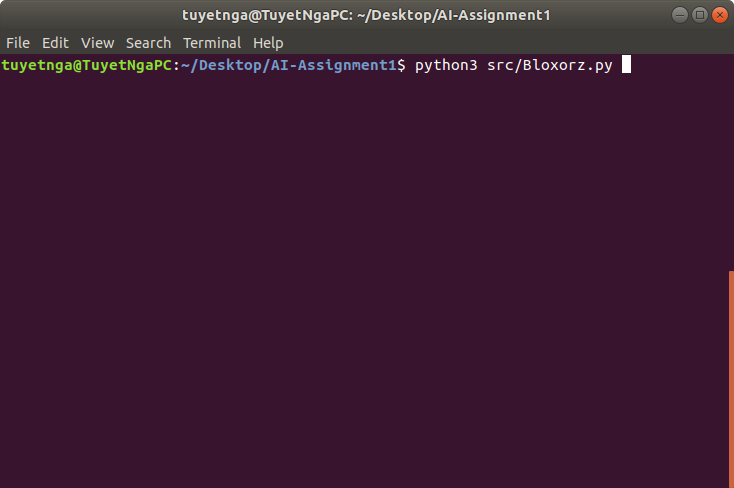
\includegraphics[width=10cm]{Images/depth1.png}
		\end{center}
		\caption{\label{fig:depth1}}
	\end{figure}
\end{center}
\begin{flushleft}
	\hspace{2 cm} Bước 2: Nhập bàn muốn chơi
\end{flushleft}
\begin{center}
	\begin{figure}[htp]
		\begin{center}
			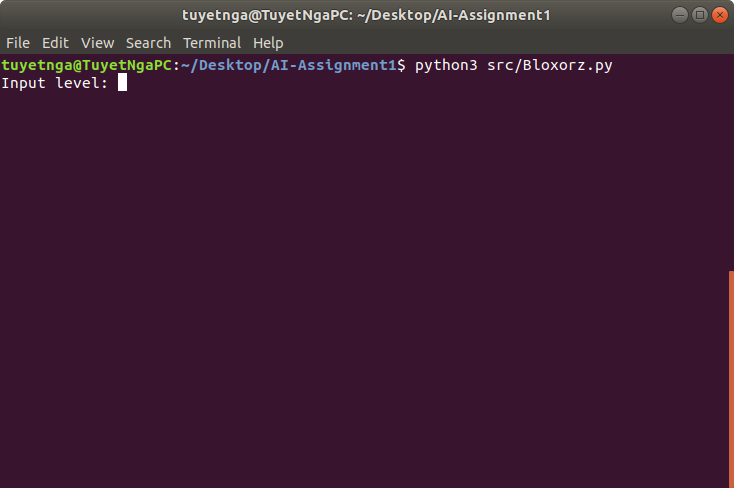
\includegraphics[width=10cm]{Images/depth2.png}
		\end{center}
		\caption{\label{fig:depth2}}
	\end{figure}
\end{center}
\newpage
\begin{flushleft}
	\hspace{3 cm} Bước 3: Nhập 1 để chọn giải thuật Breadth First Search
\end{flushleft}
\begin{center}
	\begin{figure}[htp]
		\begin{center}
			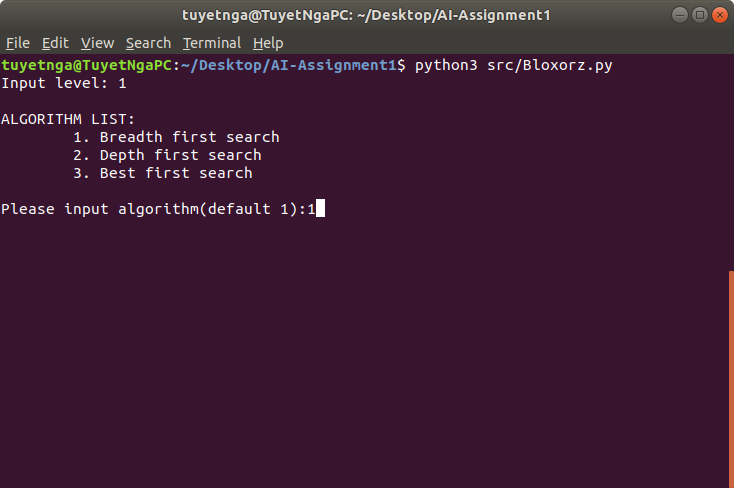
\includegraphics[width=10cm]{Images/breadth1.png}
		\end{center}
		\caption{\label{fig:breadth1}}
	\end{figure}
\end{center}
\begin{flushleft}
	\hspace{2 cm}	Bước 4: Xem demo step-by-step và xuất bước chạy rõ hơn sau khi tìm được kết quả
\end{flushleft}
\begin{center}
	\begin{figure}[htp]
		\begin{center}
			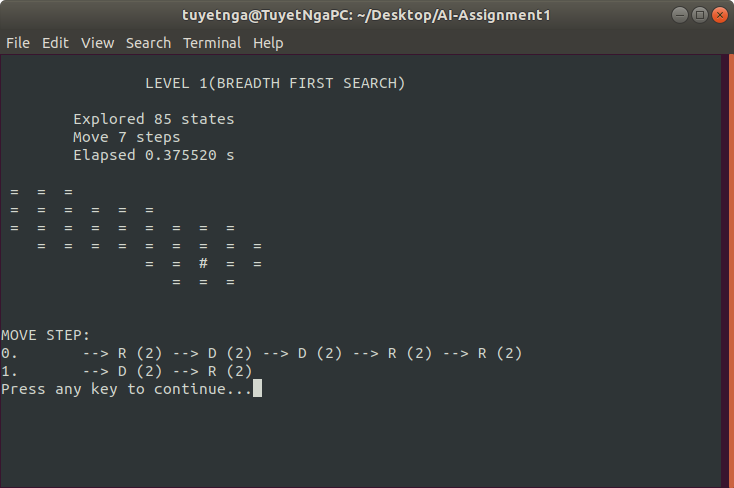
\includegraphics[width=10cm]{Images/breadth3.png}
		\end{center}
		\caption{\label{fig:breadth3}}
	\end{figure}
\end{center}
\newpage

\section{Best First Search}
\subsection{Giải thuật}
\begin{flushleft}
	\hspace{2 cm}	def best\_first\_search(initState):\\
	\hspace{3 cm}	initState.getMap().name += "(best first search)"\\
	\hspace{3 cm}	counter = 0\\
	\hspace{3 cm}	queue = PriorityQueue()\\
	\hspace{3 cm}	explored = list()\\
	\hspace{3 cm}	queue.put(initState)\\
	\hspace{3 cm}	while not queue.empty():\\
	\hspace{4 cm}	state = queue.get()\\
	\hspace{4 cm}	check, value = state.isGoal()\\
	\hspace{4 cm}	counter += 1\\
	\hspace{4 cm}	if check == True:\\
	\hspace{5 cm}	if value == None:\\
	\hspace{6 cm}	return [state, counter]\\
	\hspace{4 cm}	explored.append(state)\\
	\hspace{4 cm}	children = nextState(state)\\
	\hspace{4 cm}	for i in children:\\
	\hspace{5 cm}	if i not in explored:\\
	\hspace{6 cm}	queue.put(i)\\
	\hspace{3 cm}	return [initState, -1]\\
\end{flushleft}
\subsection{Hàm lượng giá}
\begin{flushleft}
\hspace{1 cm}	Hàm lượng giá tính khoảng cách từ điểm hiện tại tới mục tiêu cần tìm\\
\hspace{2 cm}	def distance(self):\\
\hspace{3 cm}	A = self.block.A\\
\hspace{3 cm}	g = self.lsGoal[0]\\
\hspace{3 cm}	if self.block.control == A and self.goalA:\\
\hspace{4 cm}	g = self.goalA[0]\\
\hspace{3 cm}	elif self.block.control == self.block.B and self.goalB:\\
\hspace{4 cm}	A = self.block.B\\
\hspace{4 cm}	g = self.goalB[0]\\
\hspace{3 cm}	if g.type == CHANGECONTROL:\\
\hspace{4 cm}	g = self.lsGoal[0]\\
\hspace{3 cm}	vectorAG = [g.x - A.x, g.y - A.y]\\
\hspace{3 cm}	return sqrt(vectorAG[0]**2 + vectorAG[1]**2)\\
\end{flushleft}
\subsection{Kết quả chi tiết từng bài}
\begin{center}
	\begin{tabular}{|c|r|c|c|}
		\hline
		Bài & Thời gian tìm kiếm kết quả & Bước chuyển & Trạng thái \\ \hline
		1   & 0.030900 s	& 7		& 9 \\ \hline
		2   & 0.221260 s	& 18	& 39 \\ \hline
		3	& 0.298219 s	& 30	& 53 \\ \hline
		4 	& 0.846096 s	& 39	& 86 \\ \hline
		5	& 2.576809 s	& 34	& 218 \\ \hline
		6	& 0.893582 s	& 40	& 87 \\ \hline
		7	& 1.480511 s	& 59	& 186 \\ \hline
		8	& 0.106365 s	& 11	& 14 \\ \hline
		9	& 6.626361 s	& 42	& 1013 \\ \hline
		10	& 31.932690 s	& 58	& 2336 \\ \hline
		11	& 0.609098 s	& 47	& 80 \\ \hline
		12	& 3.656315 s	& 66	& 355 \\ \hline
		13	& 0.858556 s	& 48	& 87 \\ \hline
		14	& 4.849752 s	& 72	& 497 \\ \hline
		15	& 6.472636 s	& 84	& 609 \\ \hline
		16	& 0.769421 s	& 38	& 112 \\ \hline
		17	& 6.513172 s	& 109	& 602 \\ \hline
		18	& 1.998310 s	& 90	& 225 \\ \hline
		19	& 1.351635 s	& 67	& 143 \\ \hline
		20	& 5.236975 s	& 0		& -1  \\ \hline
		21	& 1.302634 s	& 71	& 139 \\ \hline
		22	& 2.916878 s	& 81	& 316 \\ \hline
		23	& 5.284086 s	& 12820	& 7268 \\ \hline
		24	& 1.962009 s	& 82	& 251 \\ \hline
		25	& 2.109535 s	& 55	& 234 \\ \hline
		26	& 83.173022 s	& 0		& -1 \\ \hline
		27	& 2.490003 s	& 71	& 254 \\ \hline
		28	& 4.411172 s	& 110	& 381 \\ \hline
		29	& 29.840586 s	& 127	& 2156 \\ \hline
		30	& 4.848795 s	& 114	& 481 \\ \hline
		31	& 8.243943 s	& 92	& 770 \\ \hline
		32	& 5.548439 s	& 129	& 625 \\ \hline
		33	& 2.770999 s	& 80	& 277 \\ \hline
	\end{tabular}	
\end{center}
\newpage
\subsection{Cách chạy} 
\begin{flushleft}
	\hspace{2 cm}	Bước 1: Chạy lệnh python3 src/Bloxor.py để vào chương trình
\end{flushleft}
\begin{center}
	\begin{figure}[htp]
		\begin{center}
			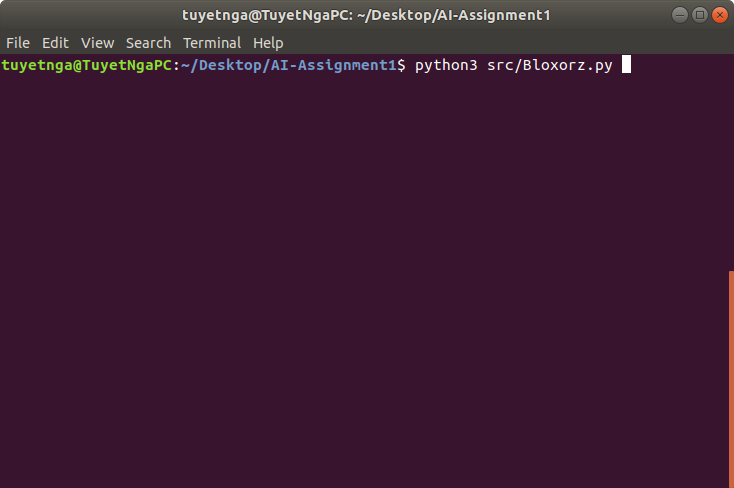
\includegraphics[width=10cm]{Images/depth1.png}
		\end{center}
		\caption{\label{fig:depth1}}
	\end{figure}
\end{center}
\begin{flushleft}
	\hspace{2 cm} Bước 2: Nhập bàn muốn chơi
\end{flushleft}
\begin{center}
	\begin{figure}[htp]
		\begin{center}
			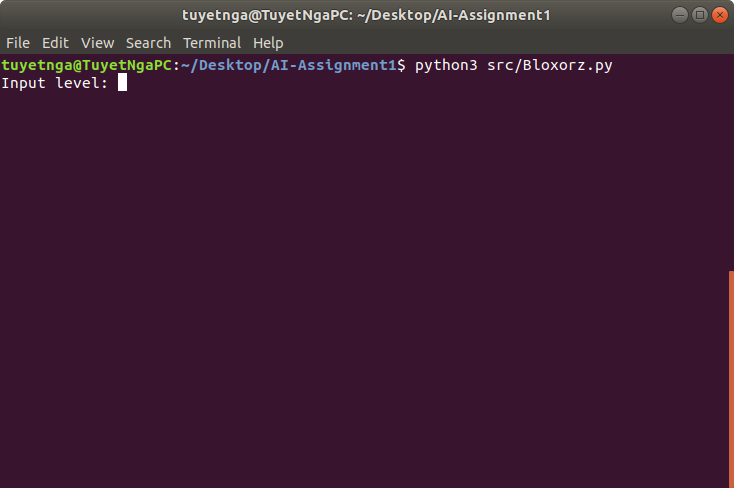
\includegraphics[width=10cm]{Images/depth2.png}
		\end{center}
		\caption{\label{fig:depth2}}
	\end{figure}
\end{center}
\newpage
\begin{flushleft}
	\hspace{3 cm} Bước 3: Nhập 3 để chọn giải thuật Best First Search
\end{flushleft}
\begin{center}
	\begin{figure}[htp]
		\begin{center}
			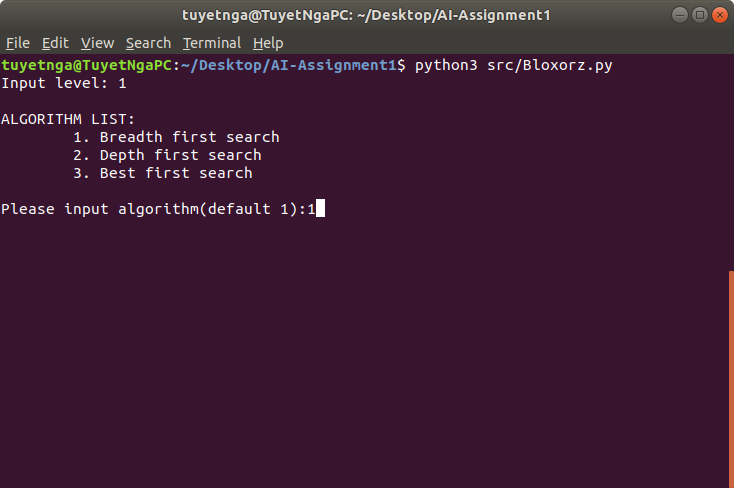
\includegraphics[width=10cm]{Images/breadth1.png}
		\end{center}
		\caption{\label{fig:best1}}
	\end{figure}
\end{center}
\begin{flushleft}
	\hspace{2 cm}	Bước 4: Xem demo step-by-step và xuất bước chạy rõ hơn sau khi tìm được kết quả
\end{flushleft}
\begin{center}
	\begin{figure}[htp]
		\begin{center}
			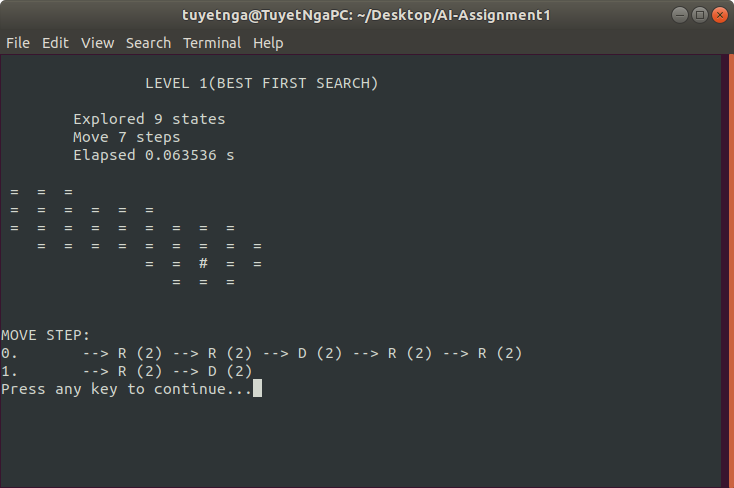
\includegraphics[width=10cm]{Images/best3.png}
		\end{center}
		\caption{\label{fig:best3}}
	\end{figure}
\end{center}
\newpage
\section {Hiệu năng về thời gian của Best First Search so với Breadth First Search }
\begin{center}
	\begin{tabular}{|c|r|c|c|r|c|c|r|}
		\hline
	\multirow{2}{1 cm}{ Bài} & \multicolumn{3}{|c|}{Breadth First Search} & \multicolumn{3}{|c|}{Best First Search} & \multirow{2}{1 cm}{Hiệu năng} \\	
	& Thời gian  & Bước & Trạng thái & Thời gian & Bước & Trạng thái & \\ \hline
		1   & 0.346270 s	& 7		& 85	& 0.030900 s	& 7		& 9 	& 8.923672 \\ \hline
		2   & 4.163358 s	& 17	& 626	& 0.221260 s	& 18	& 39	& 5.314460 \\ \hline
		3	& 1.073998 s	& 19	& 174	& 0.298219 s	& 30	& 53	& 27.767183 \\ \hline
		4 	& 0.904767 s	& 28	& 99	& 0.846096 s	& 39	& 86	& 93.610841 \\ \hline
		5	& 3.377141 s	& 34	& 319	& 2.576809 s	& 34	& 218	& 76.301493 \\ \hline
		6	& 2.277367 s	& 35	& 204	& 0.893582 s	& 40	& 87	& 39.237505 \\ \hline
		7	& 2.427308 s	& 45	& 271	& 1.480511 s	& 59	& 186	& 60.993949 \\ \hline
		8	& 0.906574 s	& 11	& 108	& 0.106365 s	& 11	& 14	& 11.732633 \\ \hline
		9	& 1.094362 s	& 24	& 199	& 6.626361 s	& 42	& 1013	& 605.499917 \\ \hline
		10	& 27.803828 s	& 57	& 2219	& 31.932690 s	& 58	& 2336	& 114.849977 \\ \hline
		11	& 0.751215 s	& 47	& 89	& 0.609098 s	& 47	& 80	& 81.081714 \\ \hline
		12	& 4.972121 s	& 60	& 556	& 3.656315 s	& 66	& 355	& 73.536324 \\ \hline
		13	& 2.421999 s	& 46	& 235	& 0.858556 s	& 48	& 87	& 35.448239 \\ \hline
		14	& 6.123488 s	& 67	& 618	& 4.849752 s	& 72	& 497	& 79.199175 \\ \hline
		15	& 4.726335 s	& 64	& 490	& 6.472636 s	& 84	& 609	& 136.948312 \\ \hline
		16	& 2.966731 s	& 40	& 342	& 0.769421 s	& 38	& 112	& 25.934977 \\ \hline
		17	& 14.307251 s	& 106	& 1379	& 6.513172 s	& 109	& 602	& 45.523574 \\ \hline
		18	& 3.665601 s	& 92	& 364	& 1.998310 s	& 90	& 225	& 54.515208 \\ \hline
		19	& 3.103062 s	& 67	& 296	& 1.351635 s	& 67	& 143	& 43.558105 \\ \hline
		20	& 3.309927 s	& 61	& 347	& 5.236975 s	& 0		& -1	& 0  \\ \hline
		21	& 3.996603 s	& 71	& 395	& 1.302634 s	& 71	& 139	& 32.59353 \\ \hline
		22	& 6.003093 s	& 77	& 610	& 2.916878 s	& 81	& 316	& 48.589585 \\ \hline
		23	& 23.857360 s	& 75	& 2066	& 5.284086 s	& 12820	& 7268	& 22.148662 \\ \hline
		24	& 1.112096 s	& 57	& 150	& 1.962009 s	& 82	& 251	& 176.424427 \\ \hline
		25	& 3.084451 s	& 55	& 295	& 2.109535 s	& 55	& 234	& 68.39256 \\ \hline
		26	& 8.722139 s	& 110	& 956	& 83.173022 s	& 0		& -1	& 0 \\ \hline
		27	& 4.643386 s	& 71	& 403	& 2.490003 s	& 71	& 254	& 53.624726 \\ \hline
		28	& 11.883237 s	& 100	& 1102	& 4.411172 s	& 110	& 381	& 37.120963 \\ \hline
		29	& 9.317949 s	& 110	& 947	& 29.840586 s	& 127	& 2156	& 320.248437 \\ \hline
		30	& 13.321815 s	& 114	& 1077	& 4.848795 s	& 114	& 481	& 36.397405 \\ \hline
		31	& 8.140459 s	& 86	& 759	& 8.243943 s	& 92	& 770	& 101.271231 \\ \hline
		32	& 9.089880 s	& 129	& 1051	& 5.548439 s	& 129	& 625	& 61.039739\\ \hline
		33	& 3.757065 s	& 65	& 362	& 2.770999 s	& 80	& 277	& 73.754353\\ \hline
	\end{tabular}	
\end{center}
\subsection{So sánh hiệu năng Best First Search so với Breadth First Search}
\coler{black}
\begin{center}
	\begin{quotation}
		\textbullet \hspace{0.25 cm} Thời gian trung bình là 80.3509964, thời gian tìm kiếm lời giải ít hơn so với Breadth First Search do nó luôn tìm đường đến mục tiêu gần nhất $\Rightarrow$ Thời gian tối ưu hơn \\
		\textbullet	\hspace{0.25 cm}	Trạng thái trung bình là 20.1818182, đa số trạng thái của Best First Search ít hơn so với Breadth First Search nên về bộ nhớ sẽ chứa ít hơn, tuy nhiên do vài bài bị dính vấn đề tôi ưu cục bộ nên trạng thái nhiều hơn dẫn đến tổng số trạng thái trung bình của Best First Search sẽ nhiều hơn Breadth First Search $\Rightarrow$ Nhìn tổng quát thì Best First Search vẫn sẽ tốt hơn\\
		\textbullet \hspace{0.25 cm} Mà nhìn chung Breadth First Search sẽ tối ưu hơn so với Depth First Search\\
		$\Rightarrow$ Vậy Best First Search tối ưu về thời gian và bộ nhớ hơn so với Breadth First Search và Depth First Search
	\end{quotation}	
\end{center}
\subsection{Cách chạy}
\begin{description}
	\item \hspace{1 cm}	Chạy lệnh python3 src/Bloxors.py runall để chạy hết các màn game 1 lượt để xuất ra kết quả các trạng thái, bước chuyển và thời gian chạy giữa Best First Search và Breadth First Search (Riêng Depth First Search do phải giới hạn chiều dài của cây nên khó so sánh hết các màn 1 lần được). Kết quả sẽ hiện trên file result.txt như hình dưới:
\end{description}
\newpage
\begin{center}
	\begin{figure}[htp]
		\begin{center}
			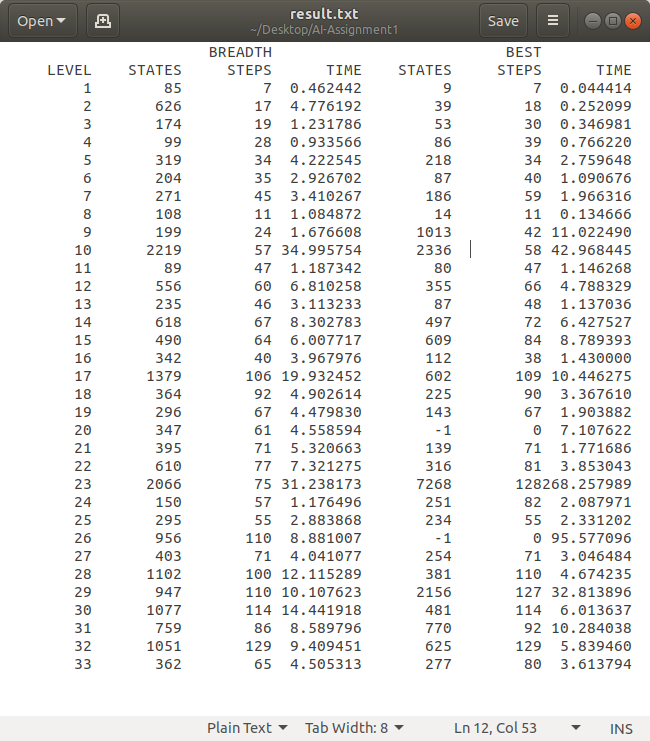
\includegraphics[width=10cm]{Images/ssBFS_va_BRFS.png}
		\end{center}
		\caption{\label{fig:ssBFS_va_BRFS}}
	\end{figure}
\end{center}

\section{Tham khảo}
\begin{flushleft}
	\hspace{2 cm} \textbullet \hspace{0.5 cm} Tài liệu học tập của môn học \\
	\hspace{2 cm} \textbullet \hspace{0.5 cm} \url{http://en.wikipedia.org/wiki/Depth-first\_search} \\
	\hspace{2 cm} \textbullet \hspace{0.5 cm} \url{http://en.wikipedia.org/wiki/Breadth-first\_search} \\
	\hspace{2 cm} \textbullet \hspace{0.5 cm} \url{http://en.wikipedia.org/wiki/Hill\_climbing} \\
	\hspace{2 cm} \textbullet \hspace{0.5 cm} \url{http://www.coolmath-games.com/0-bloxorz} \\
\end{flushleft}
\end{document}


